\newpage
\section{Four bit adder - using signed/unsigned logic}

\begin{enumerate}
	\item[1)]
	Vi laver en unsigned adder i dataflow style som vist på figur \ref{fig:4bitUnsignedAdder}. Da input og output skal være af std logic vector typen, og vi skal bruge + operatoren, bliver vi nødt til at konvertere til unsigned først. Se Kode \ref{lst:4bitUnsignedDataflowCode}\\
	
	\begin{figure}[H]
		\centering
		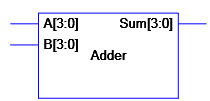
\includegraphics[scale=0.5]{pictures/Oevelse3/4bit_unsigned_adder.jpg}
		\caption{Four bit unsigned adder}
		\label{fig:4bitUnsignedAdder}
	\end{figure}
	
	\begin{lstlisting}[caption={Four bit unsigned adder Dataflow VHDL kode},label={lst:4bitUnsignedDataflowCode}]
	library ieee;
	use ieee.std_logic_1164.all;
	use ieee.numeric_std.all;
	
	entity unsigned_adder is
	port (a: in std_logic_vector (3 downto 0);
	b: in std_logic_vector (3 downto 0);
	sum: out std_logic_vector (3 downto 0));
	end unsigned_adder;
	
	architecture dataflow of unsigned_adder is
	begin
	
	sum <= std_logic_vector(unsigned(a) + unsigned(b));
	end dataflow;
	\end{lstlisting}
	
	\item[2)]
	Vi tester nu vores kode med en functional simulation:\\
	\begin{figure}[H]	
		\centering
		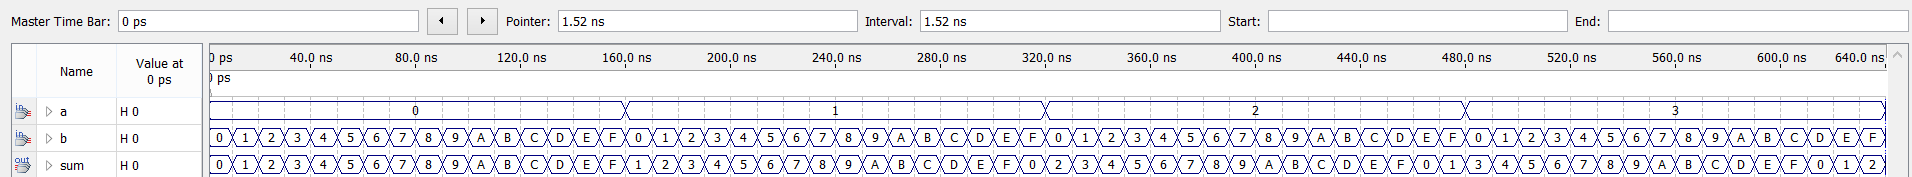
\includegraphics[scale=0.4]{pictures/Oevelse3/4bit_unsigned_adder_functional_simulation.jpeg}
		\caption{Four bit unsigned adder Functional simulation}
		\label{fig:4bitUnsignedAdderFuncSim}
	\end{figure}
\newpage
	\item[3)]
	Vi sætter nu bits til 1000 + 0100 og får det forventede resultat som det ses på Figur \ref{fig:4bitUnsignedAdder1100}\\
	\begin{figure}[H]
		
		\centering
		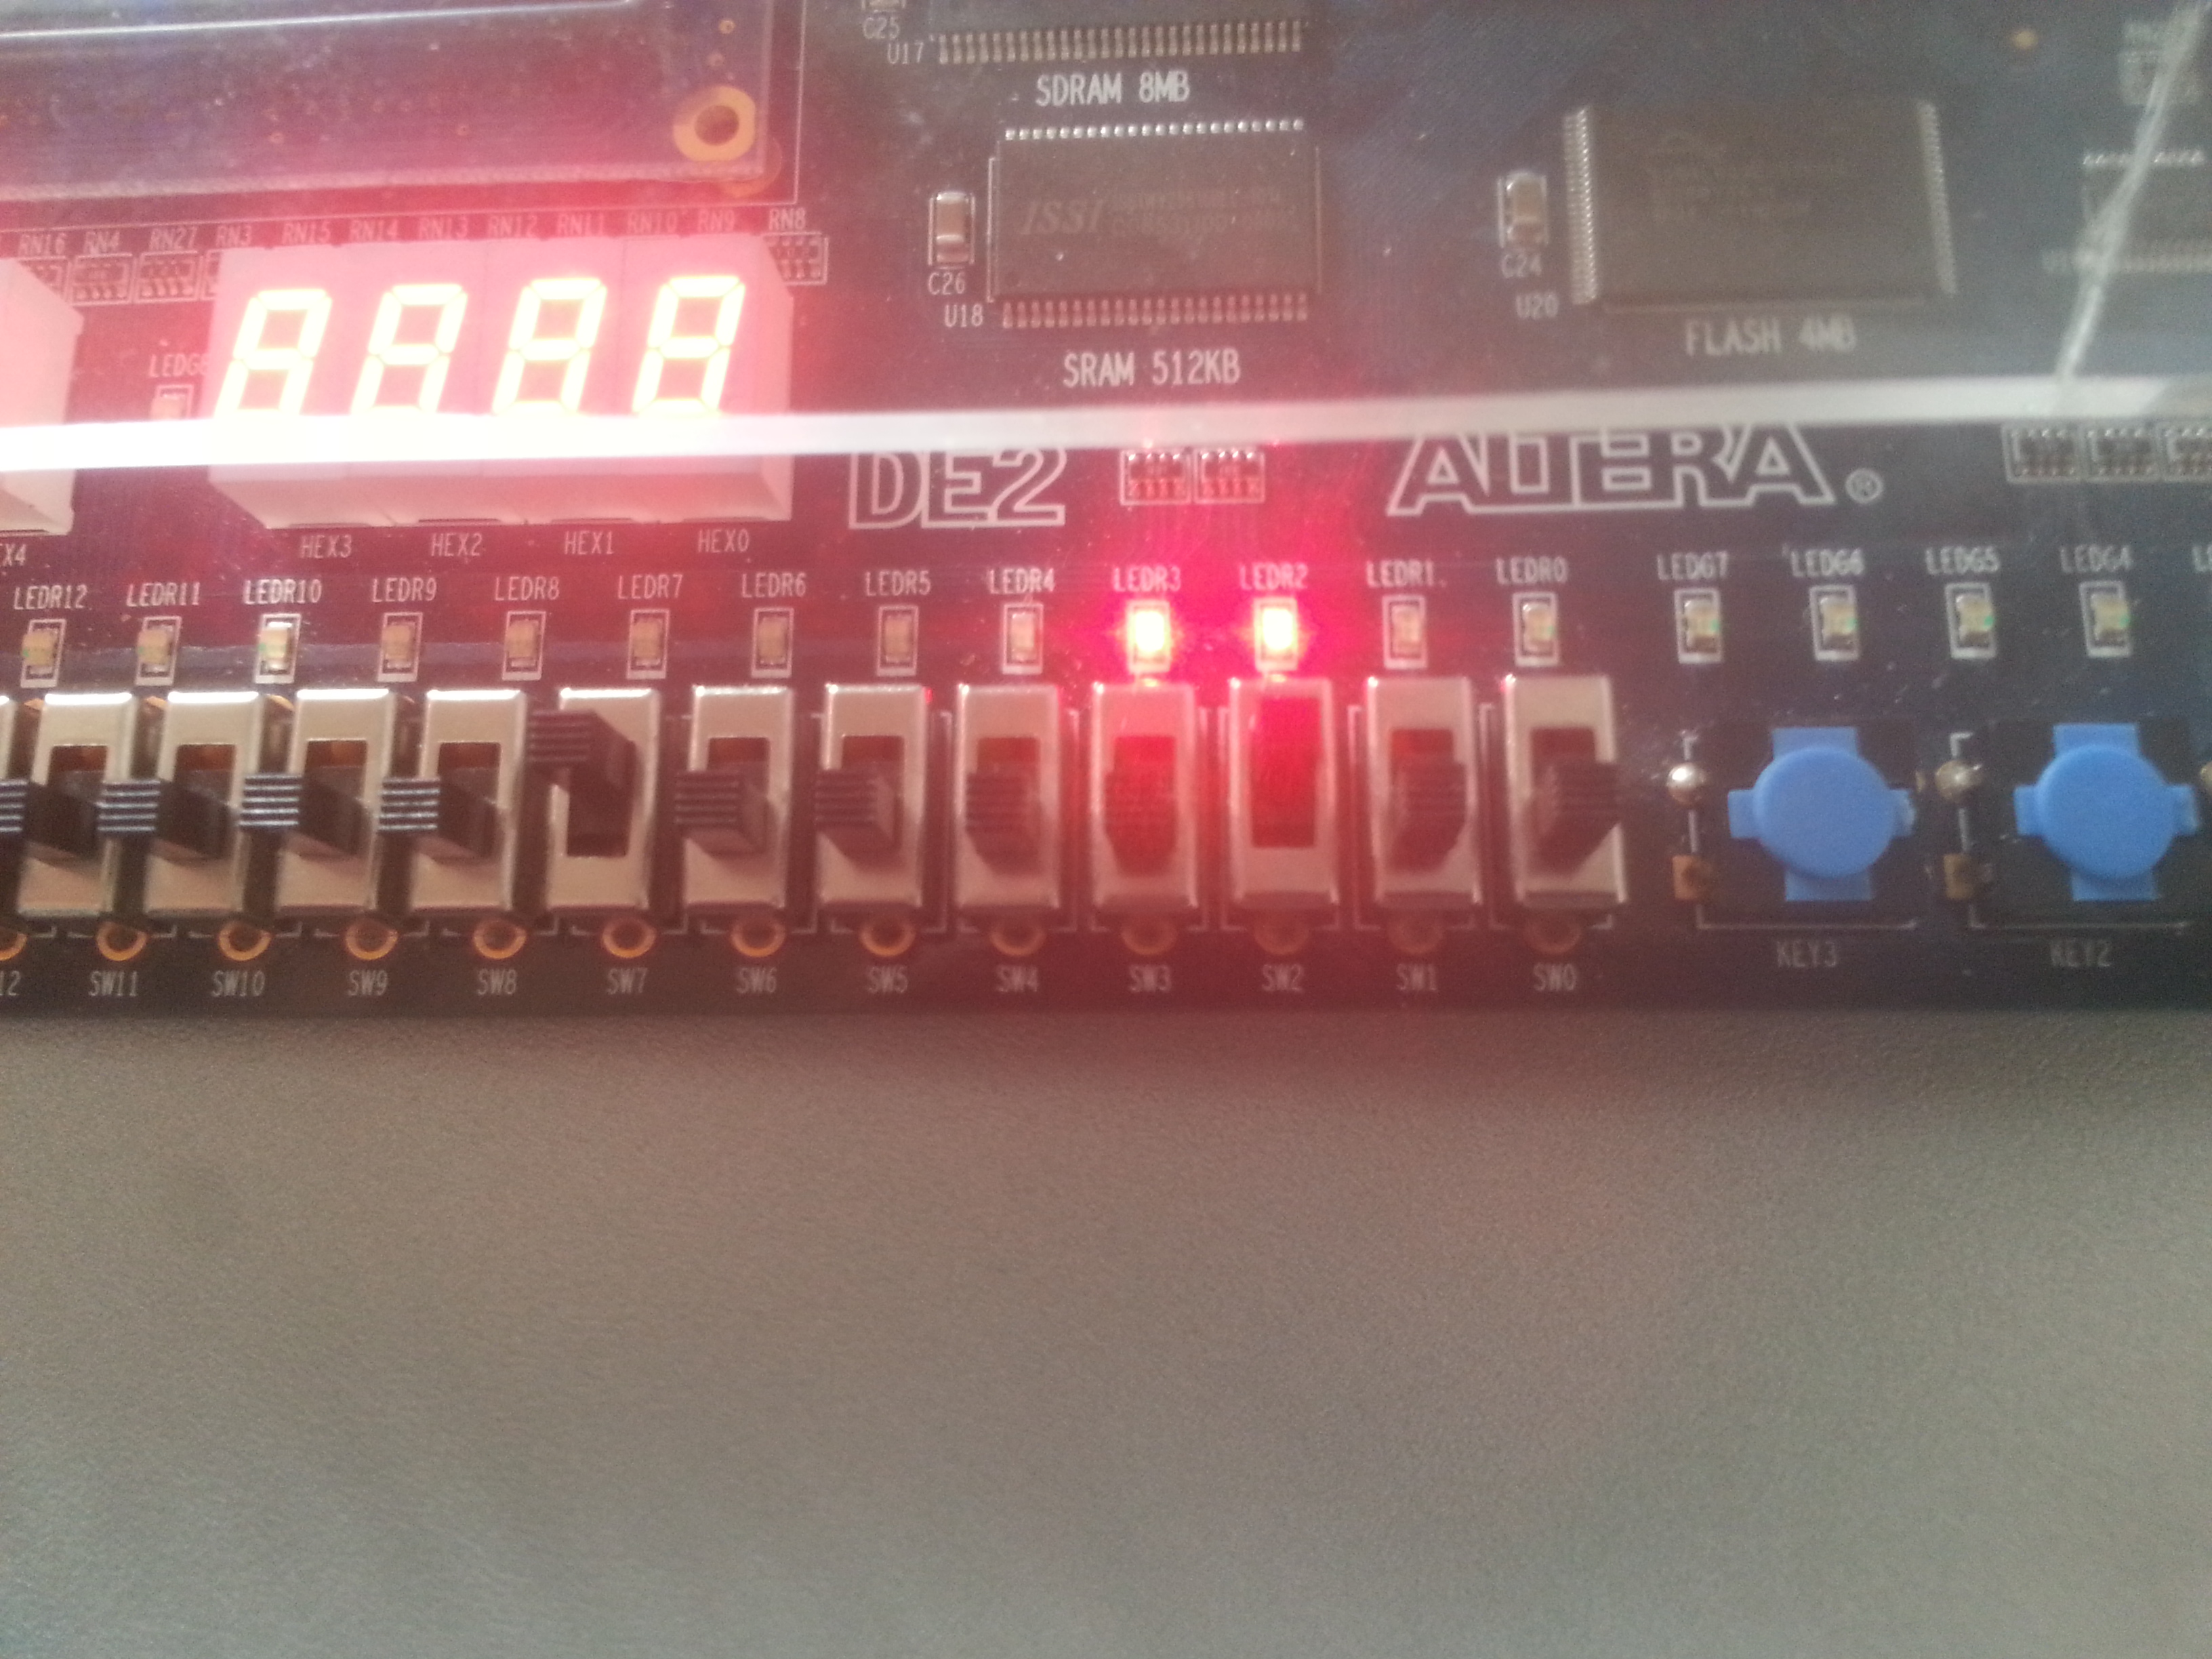
\includegraphics[width=0.8\textwidth]{pictures/Oevelse3/four_bit_unsigned_adder1.jpg}
		\caption{Four bit unsigned adder - 1000 + 0100}
		\label{fig:4bitUnsignedAdder1100}
	\end{figure}

	\item[4)]
	Vi ændrer nu koden så det bliver en signed adder som det ses i Kode \ref{lst:4bitsignedDataflowCode}. Vi tester det på vores DE2 board, og ser at der ingen forskel er på unsigned adderen og signed adderen som det ses på Figur \ref{fig:4bitSignedAdder1100}. Dette skyldes at selve bit'sne ikke er anderledes, men det er kun måden de skal tolkes på.
	
	\begin{lstlisting}[caption={Four bit signed adder Dataflow VHDL kode},label={lst:4bitsignedDataflowCode}]
	library ieee;
	use ieee.std_logic_1164.all;
	use ieee.numeric_std.all;
	
	entity unsigned_adder is
	port (a: in std_logic_vector (3 downto 0);
	b: in std_logic_vector (3 downto 0);
	sum: out std_logic_vector (3 downto 0));
	end unsigned_adder;
	
	architecture dataflow of unsigned_adder is
	begin
	
	sum <= std_logic_vector(unsigned(a) + unsigned(b));
	end dataflow;
	\end{lstlisting}
	
	\begin{figure}[htpb]
		\centering
		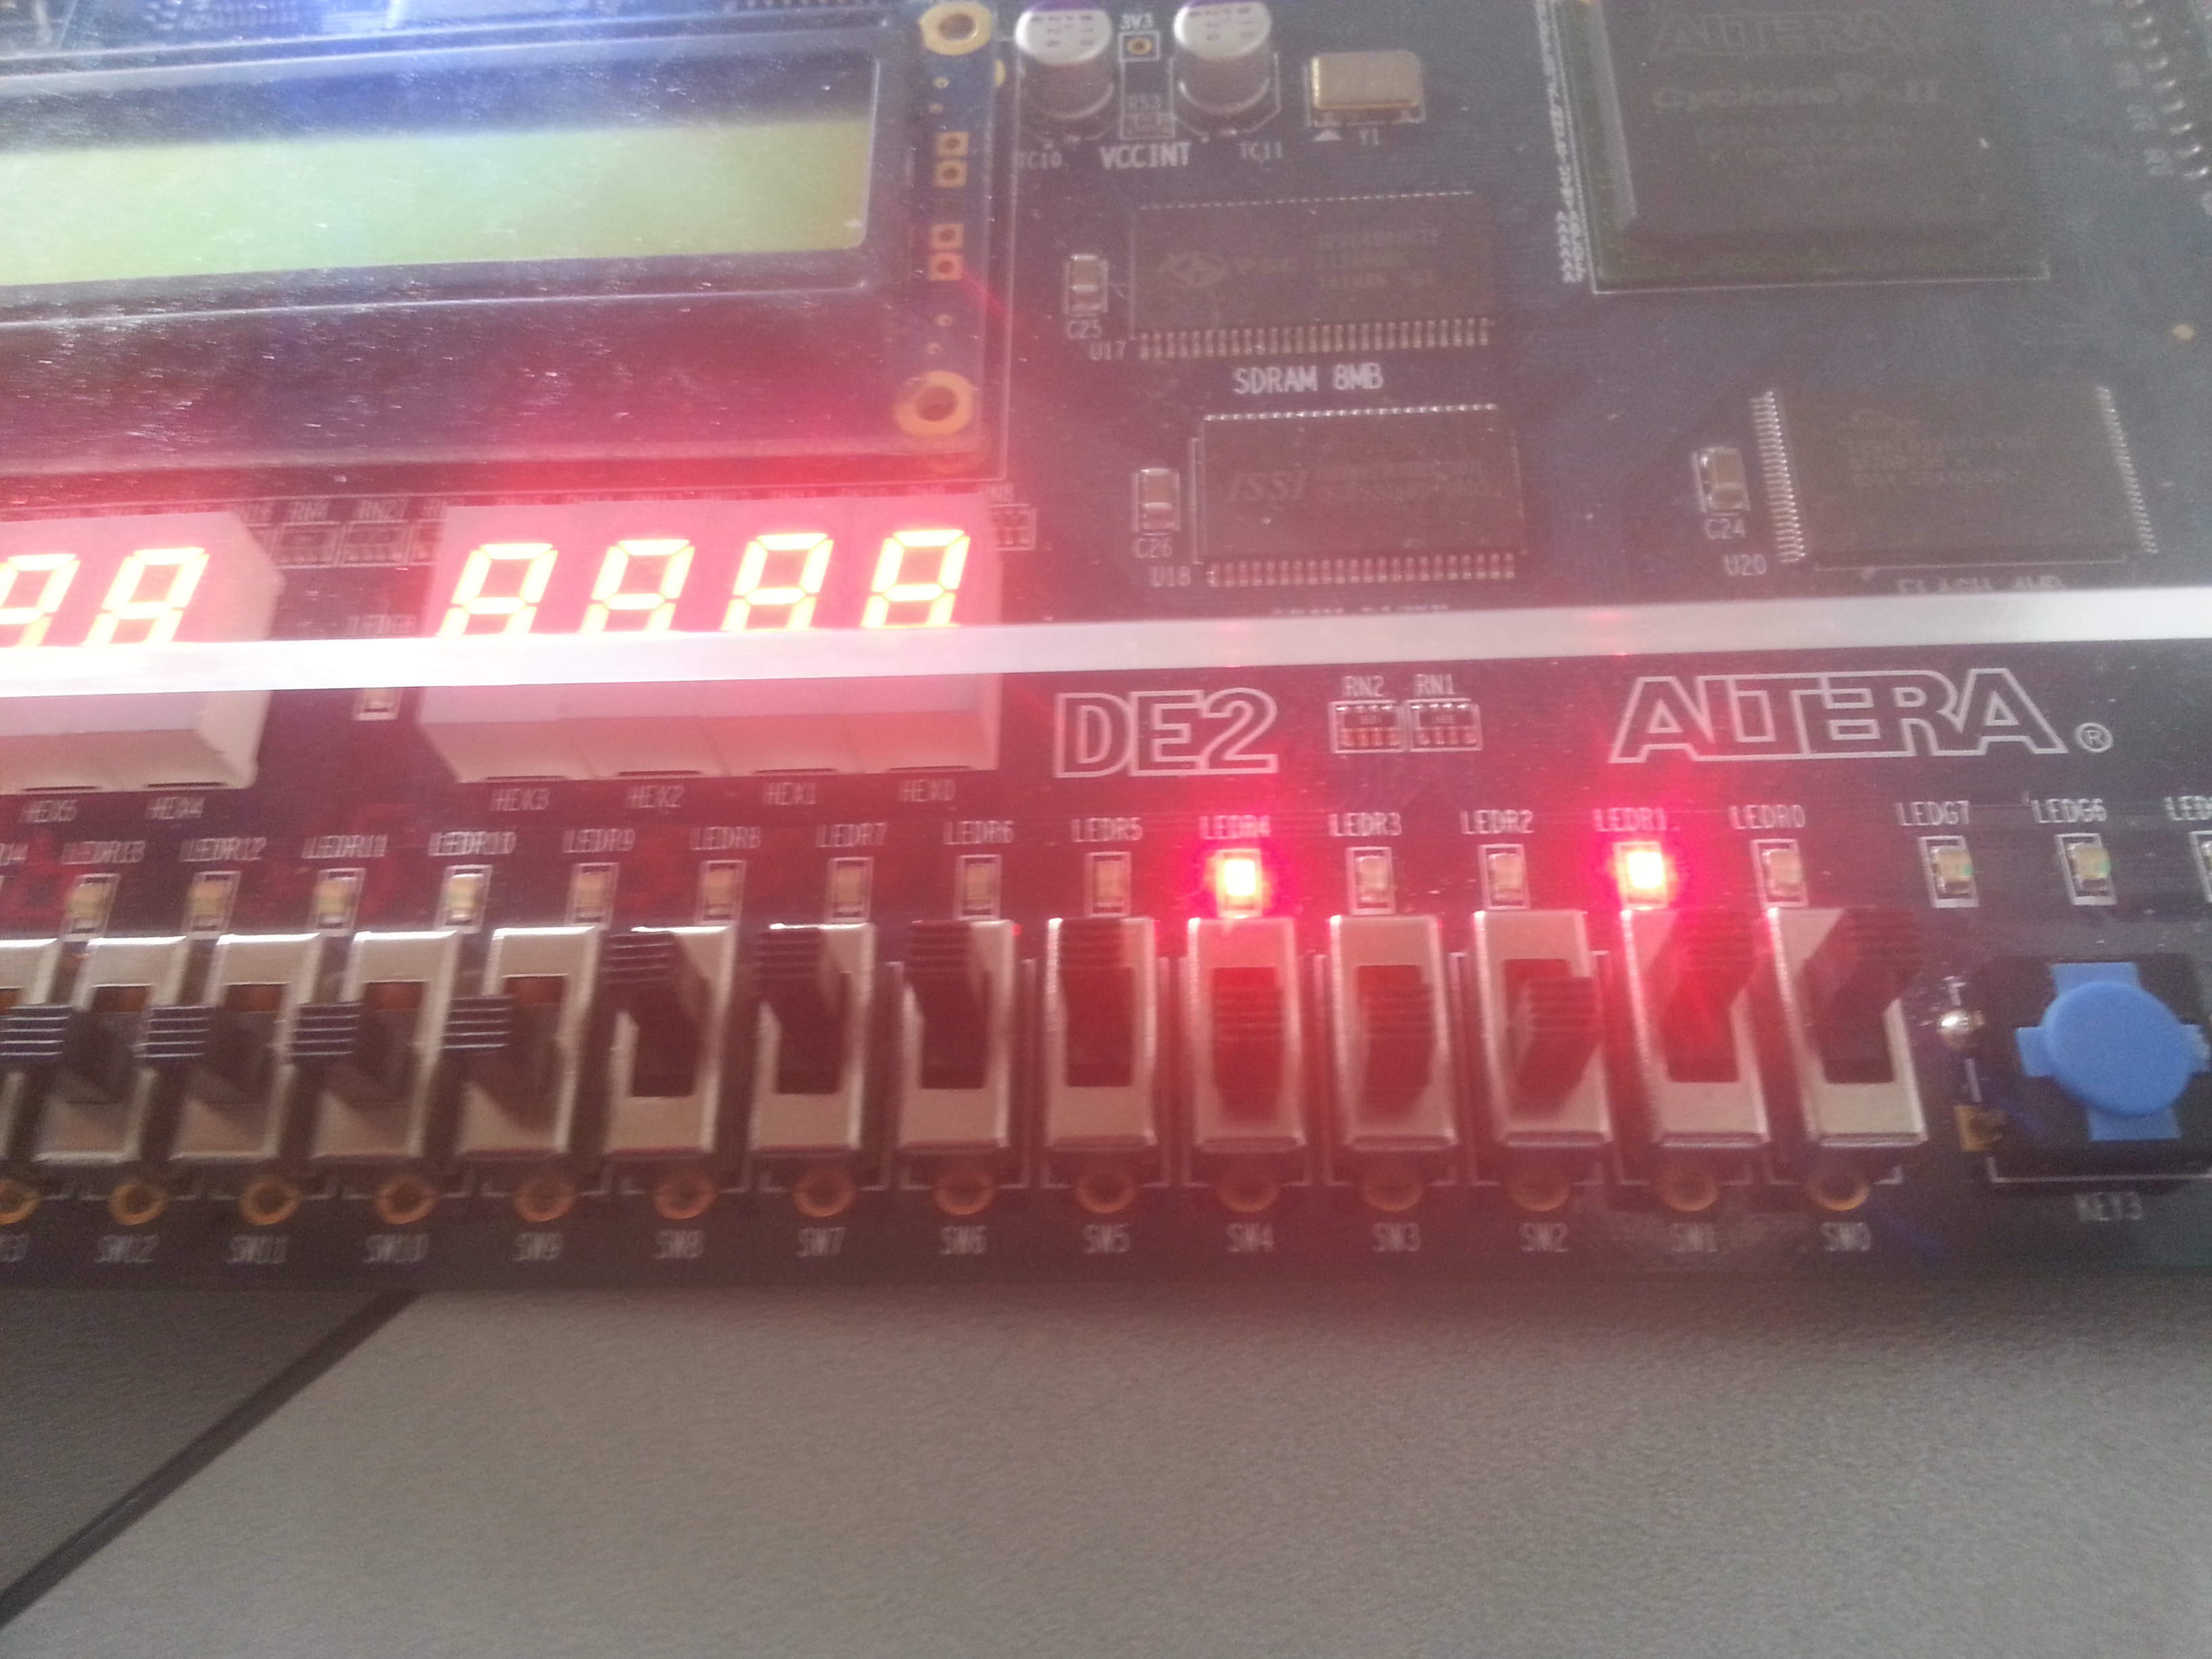
\includegraphics[width=0.8\textwidth]{pictures/Oevelse3/four_bit_signed_adder1.jpg}
		\caption{Four bit signed adder - 1000 + 0100}
		\label{fig:4bitSignedAdder1100}
	\end{figure}
	\FloatBarrier
\item[5)]
Vi laver nu vores unsigned adder om, så den også virker med et carry in, og leverer et carry out som vist på Figur \ref{fig:4bitUnsignedAdderCarry}. Vi benytter os af resize funktionen, samt laver nogle interne signaler, inden vi sender resultatet ud igen. Koden ses i Kode \ref{lst:4bitunsignedCarryDataflowCode}.
	\begin{figure}[H]
		\centering
		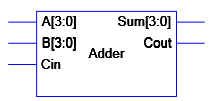
\includegraphics[scale=0.5]{pictures/Oevelse3/4bit_unsigned_adder_carry.jpg}
		\caption{Four bit unsigned adder with carry}
		\label{fig:4bitUnsignedAdderCarry}
	\end{figure}

	\begin{lstlisting}[caption={Four bit unsigned adder with carry Dataflow VHDL kode},label={lst:4bitunsignedCarryDataflowCode}]
	library ieee;
	use ieee.std_logic_1164.all;
	use ieee.numeric_std.all;
	
	entity unsigned_adder_carry is
	port (a: in std_logic_vector (3 downto 0);
	b: in std_logic_vector (3 downto 0);
	carry_in: in std_logic;
	carry_out : out std_logic_vector (0 downto 0);
	sum: out std_logic_vector (3 downto 0));
	end unsigned_adder_carry;
	
	architecture dataflow of unsigned_adder_carry is
	signal c : unsigned (3 downto 0);
	signal s : unsigned (4 downto 0);
	begin
	c <= "000" & carry_in;
	s <= resize(unsigned(a),5) + resize(unsigned(b),5) + resize(c,5) ;
	sum <= std_logic_vector(s(3 downto 0));
	carry_out <= std_logic_vector(s(4 downto 4));
	end dataflow;
	\end{lstlisting}

	\item[6)]
	Vi overfører vores adder til DE2 boardet. Her adderer vi 1110 + 0011 samt carry in = 1, og får det forventede resultat som ses på figur \ref{fig:4bitUnsignedAdderCarry10100}.
	\begin{figure}[H]
		\centering
		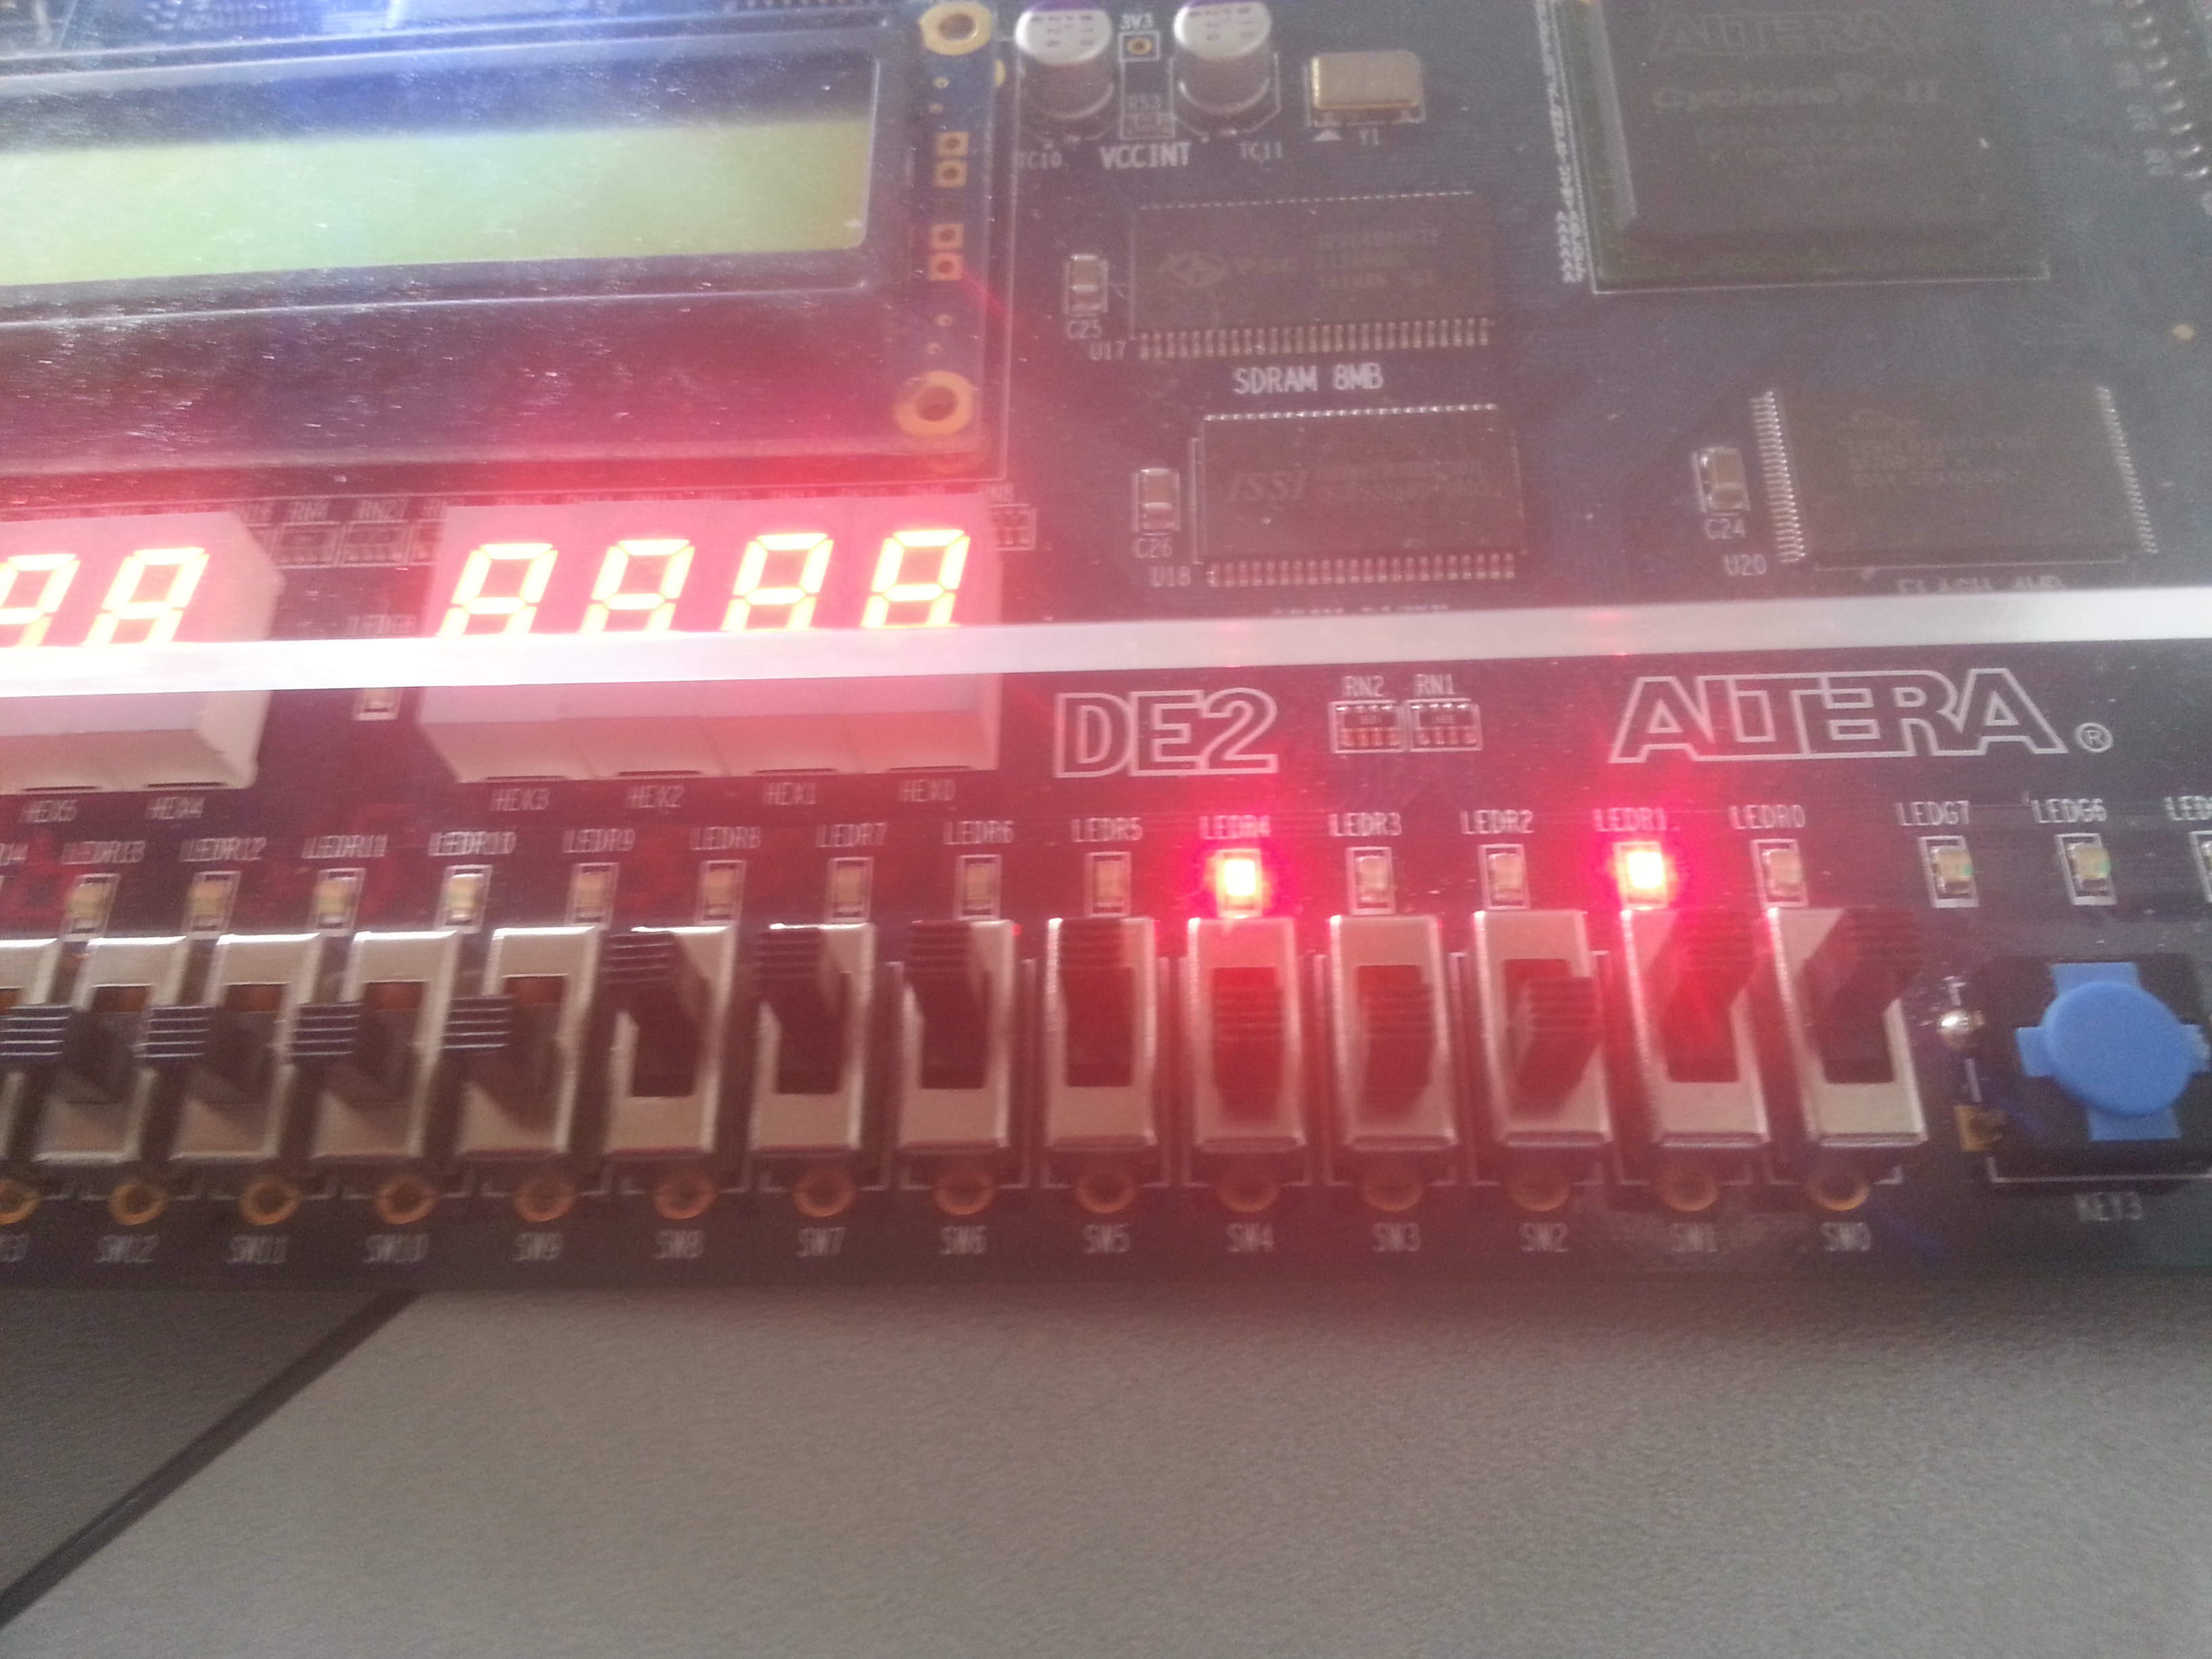
\includegraphics[width=0.8\textwidth]{pictures/Oevelse3/4bit_unsigned_adder_carry2.jpg}
		\caption{Four bit unsigned adder with carry}
		\label{fig:4bitUnsignedAdderCarry10100}
	\end{figure}
	
\end{enumerate}